\documentclass{article}
\usepackage[margin=1.25in,top=1in,bottom=1in]{geometry}
\usepackage{float}
\usepackage{setspace}
\usepackage{lineno}
\linenumbers
\linespread{2} 
\usepackage{natbib}
\bibliographystyle{abbrvnat}
\setcitestyle{authoryear,open={(},close={)}}
\usepackage{multirow}
\usepackage{graphicx}
\usepackage{hyperref}
\usepackage{rotating}
\usepackage{blindtext}
\usepackage{booktabs}
\usepackage{xcolor}
\usepackage{amsmath}
\usepackage{bbm}
\usepackage{epstopdf}
\newcommand{\ignore}[1]{}
%---------------------------------------------------------------------------------------------------------
%---------------------------------------------------------------------------------------------------------
\begin{document}
\begin{flushright}
\today
\end{flushright}
\begin{center}
\begin{LARGE}
    \textbf{Assessing the effects of date and sequence data in phylodynamics}
\end{LARGE}
\end{center}
Leo A. Featherstone$^{\ast,1}$, Sebastian Duchene$^1$, Timothy G. Vaughan$^{2,3}$\\
$^{1}$ Peter Doherty Institute for Infection and Immunity, University of Melbourne, Australia.\\
$^{2}$ Department of Biosystems Science and Engineering, ETH Zurich, Basel, Switzerland.\\
$^{3}$  Swiss Institute of Bioinformatics.\\
*email: leo.featherstone@unimelb.edu.au
%---------------------------------------------------------------------------------------------------------
%---------------------------------------------------------------------------------------------------------
%\section*{Significance Statement}
%Phylodynamic analysis almost always uses time stamped genome sequences to make epidemiological inference. However the field has lacked a transferable methods for quantifying and comparing the effects of data and genome data. Moreover, the ability to make this inference will be valuable for the future as the scale of pathogen genome sequence increases such that the question of maximising knowledge gain relative to sequencing effort comes into play. We introduce a fully transferable method to quantify the effects of date and sequence data and answer this question on a per-analysis basis.
%---------------------------------------------------------------------------------------------------------
%---------------------------------------------------------------------------------------------------------
\section*{Abstract}
Birth-death based methods are often used to infer epidemiological parameters from pathogen genomes in phylodynamics.
However, these methods also base their results on sampling time data in addition to genome sequence data.
We introduce a formal method for quantifying the relative impacts of the date and sequence components of the data.
We show that either data source can drive inference of the basic reproductive number, $R_0$, but note that the general approach can be used to investigate other phylodynamic parameters. This framework will allow practitioners to draw conclusions about which aspect of the data drive inference results, providing a path to a deeper understanding of commonly-used phylodynamic models and to better direct sequencing efforts during future outbreaks.
%---------------------------------------------------------------------------------------------------------
%---------------------------------------------------------------------------------------------------------
\section*{Introduction}
\textcolor{blue}{\begin{itemize}
    \item [\textbf{To do:}]
    \item Include post hoc value
    \item need to look at effects of data sources with increasing dataset size
    \item demands better understanding of tools we need
    \item eventual optimal sampling apparatus, but need a way to measure first
    \item Probably delete table 1
    \item Maybe: Include point about increasing sample size
    \item Maybe: Include future use of cancer phylodynamics
\end{itemize}}
Phylodynamics combines phylogenetic and epidemiological modelling to infer epidemiological dynamics from pathogen genome data \citep{du2015getting,baele2018recent,volz2013viral}. Analyses are usually conducted within a Bayesian framework, meaning that the output comprises posterior distributions for parameters of interest, such as the basic reproductive number, $R_{0}$ (i.e. the average number of secondary infections from the index case in an otherwise fully susceptible population). Input data usually consists of genome sequences and associated sample collection dates. In the case of birth-death-sampling models \citep{stadler_sampling-through-time_2010}, both sequence and date data inform the branching of inferred trees by either temporally clustering lineages or via sequence similarity.  Internal nodes are assumed to co-occur with transmission events, such that they provide information about patterns of transmission that sampling time data alone cannot \ignore{cite review when out}. Sampling times, or date data, are similar to standard epidemiological time series data while sequence data introduce the evolutionary aspect. The widely used birth-death model uses sampling times to infer a sampling rate which is also informative about transmission rates \citep{boskova2018influence,stadler2012estimating}. 

Phylodynamics is experiencing greater use than ever before since the onset of the SARS-CoV-2 pandemic. This commonly includes application to larger and more densely sequenced outbreaks than previously. While the value of pathogen genome data is now well established, an emergent question is whether inclusion of more sequence data after a point is of diminishing returns for some densely sequenced outbreaks. The answer to this question will  naturally vary with each dataset and pathogen considered, but a method to quantify the individual effects of date and sequence data presents a transferable way to address it. It would substantially broaden our understanding of the phylodynamic tools that now feature in infectious disease surveillance. It also has the potential to direct sampling efforts to future outbreaks for optimisation of knowledge gain against resource expenditure. 

Earlier work showed that sequence sampling times, referred to here as 'date data', can drive epidemiological inference under the birth-death model \citep{volz_sampling_2014, boskova2018influence, Featherstone2021Infectious}. However, each stopped short of proposing a transferable way to measure this effect in regular application. The birth-death model is most applicable to the question at hand since it includes a rate of sampling. The coalescent is another a key phylodynamic model, but it typically conditions on sampling dates which therefore precludes from a comparison of date and sequence effects. Some coalescent formulations include a sampling rate \citep{volz_sampling_2014}, however these are used less often than the birth death or standard \textcolor{blue}{Kingman coalescent. The Kingman coalescent also assumes a low sampling proportion} relative to population size such that its typical formulation would be inappropriate for many densely sequenced outbreaks \citep{boskova2018influence}, where the question of the effect of large amounts of sequence data is most relevant.

Building upon these earlier results, we introduce a theoretical framework and a new method to quantify the effect of sequence and dates for any parameter under the birth death with continuous sampling. We focus on continuous sampling because it is most relevant to how emerging outbreak data are collected. Our method quantifies and visualises the effect each data source has on the posterior distribution of epidemiological parameters of interest. It also classifies which data source is driving the inference, but crucially also provides a measure of  whether  a binary classification is meaningful. These observations are a critical addition the phylodynamic toolkit used to inform public health decisions because they clearly quantify the added-knowledge acquired from genomes in a given analysis.

\iffalse
\begin{table}[H]
\centering
\caption{Separating data to quantify effects}
\begin{tabular}{lcc}
                                    &   Dates Included                  &   Dates Excluded    \\
\midrule
Sequence Included                   &   Combined effect                 &   Sequence Effects            \\
Sequence Excluded                   &   Date effects                    &   Marginal Prior     \\
\bottomrule 
\label{tab:tab1}
\end{tabular}
\end{table}
\fi
%---------------------------------------------------------------------------------------------------------
%---------------------------------------------------------------------------------------------------------
\section*{New Methods}


\begin{figure}[H]
\centering
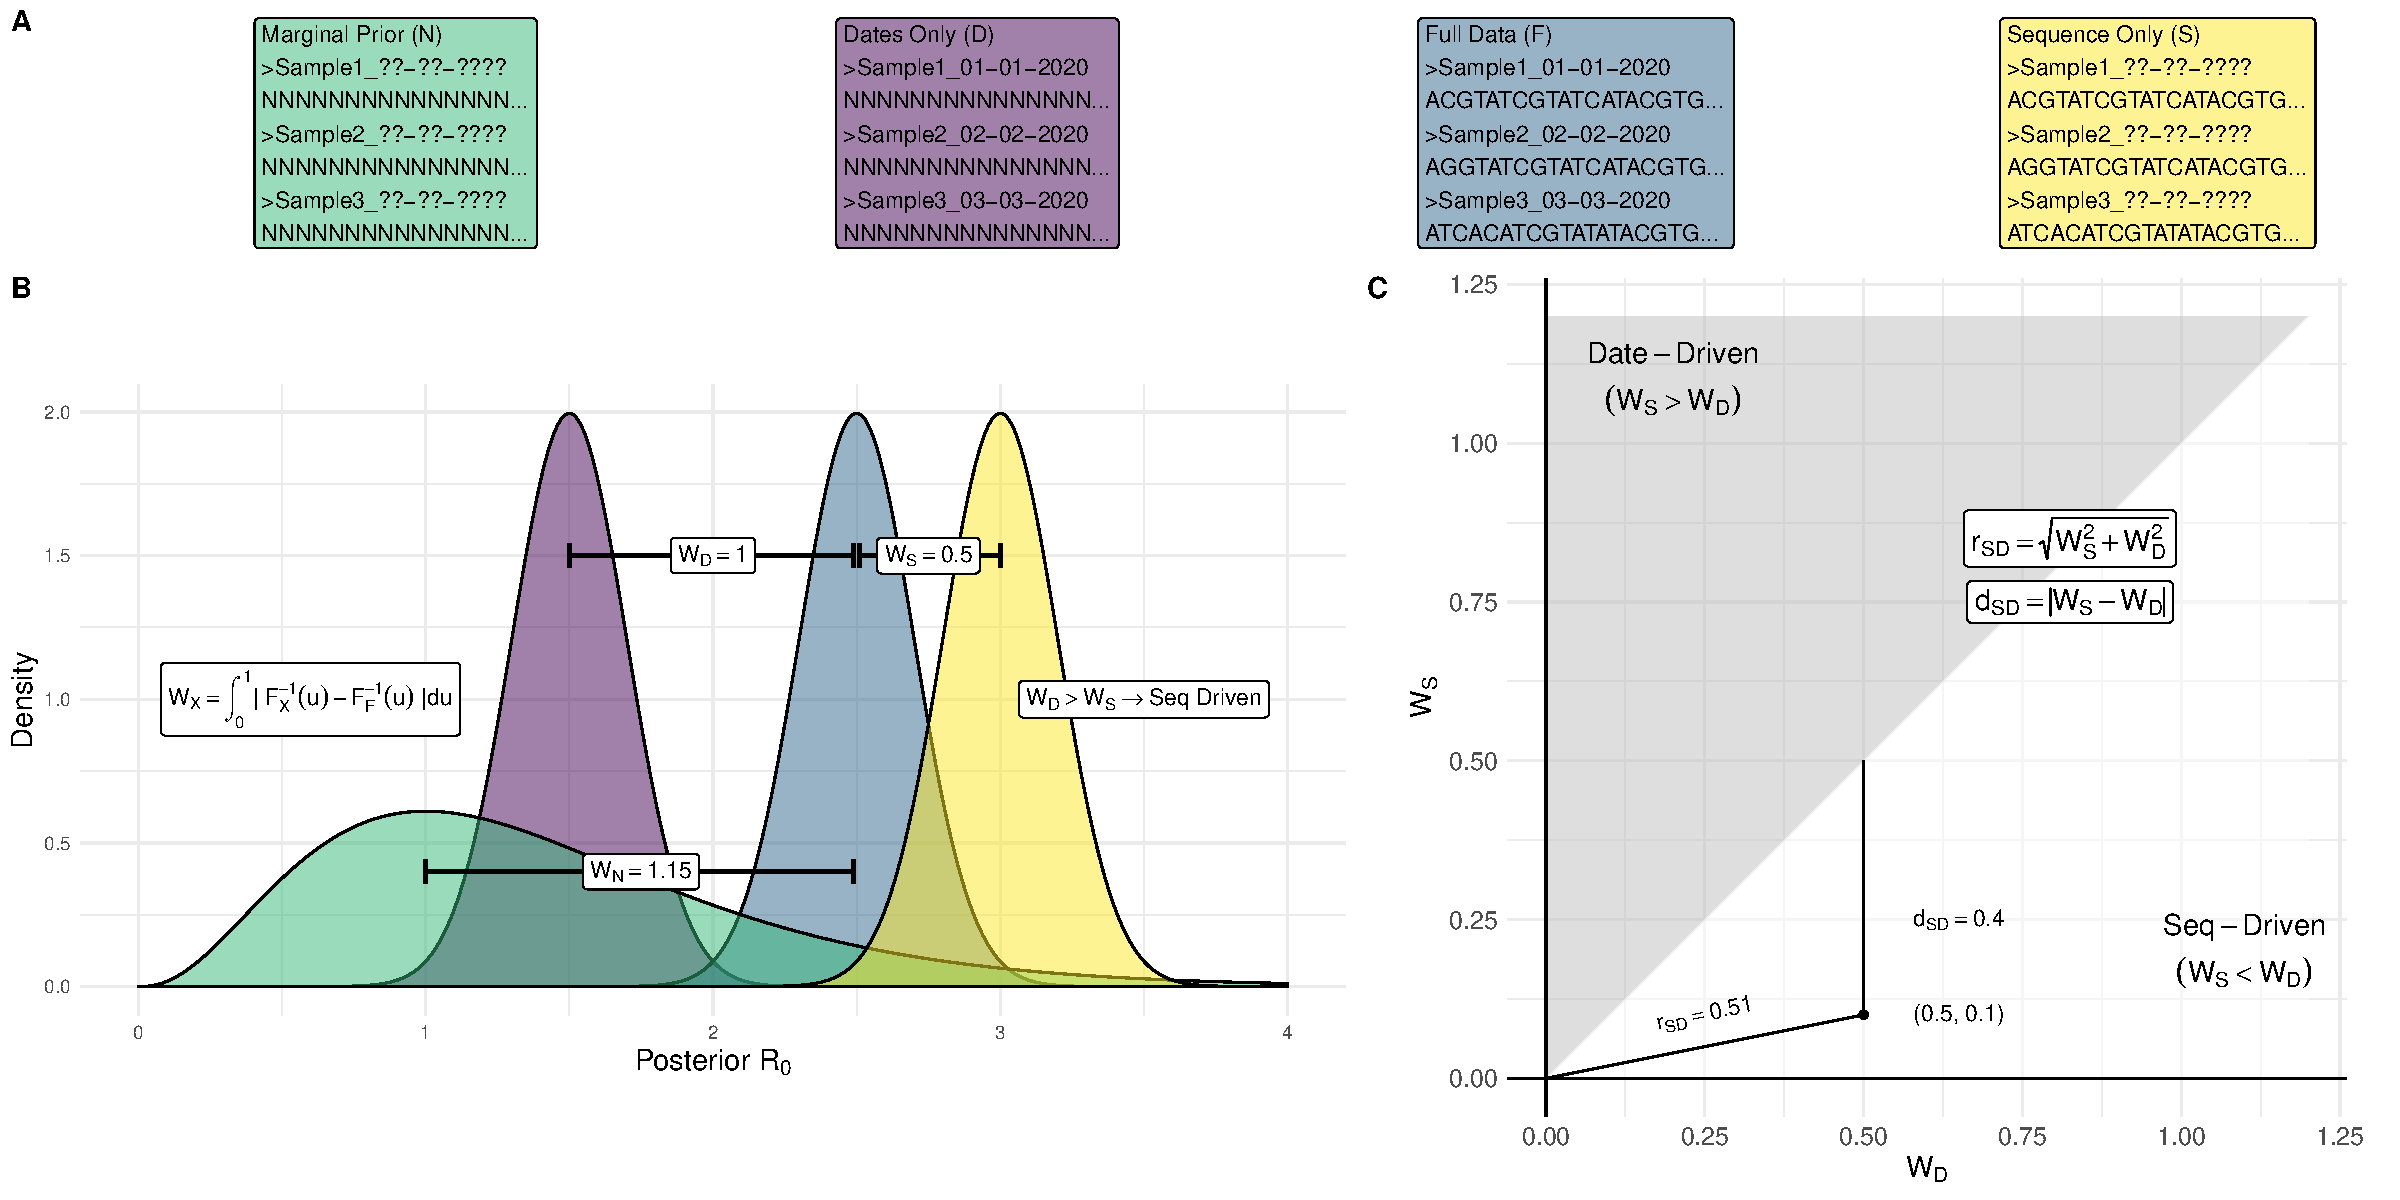
\includegraphics[width=1\linewidth]{../figures/graphicalMethods.eps}
\caption{Graphical summary of the process to quantify signal and classify signal drivers.  \textbf{A}) Coloured boxes give examples of data under each of the 4 treatments with letters in brackets giving shorthand notation for each. From left to right: \emph{Marginal Prior} results from the removal of both date and sequence data. \emph{Dates Only} includes date data while ignoring sequence data through a constant phylogenetic likelihood. This can be represented as converting all sequence characters to `N' (i.e. alignments of entirely missing data). \emph{Full data} represents the usual combination of both sequence and date data. This produces a reference distribution from which the Wasserstein metric to other posteriors is calculated. \emph{Sequence Only} corresponds to the removal and re-estimation of dates while sequence data is retained. \textbf{B}) Example posterior output for $R_0$ with colour corresponding to each treatment in \textbf{A}. The Wasserstein metric is calculated as difference in inverse distribution function of each posterior from \emph{Full Data} integrated over 0 to 1. Example values for the Wasserstein metric are given in white boxes. \textbf{C}) The plane with x and y axes $W_D$ and $W_S$ and shaded classification regions. $r_{SD}$ is the Euclidean distance from the origin to a point $(W_D, W_S)$, with higher values indicating that one or both of data and sequence data drive differing signals from the reference posterior. $d_{SD}$ is the vertical distance from a point $(W_D, W_S)$ to the line $y=x$, with points closer to this line corresponding to more similar data and sequence data effects such that classification is less meaningful. In the example, distance from the posterior under only sequence data to the full data posterior ($W_S$) is smallest, leading to classification as `Seq-Driven'.}
\label{fig:method}
\end{figure}


\subsection*{Isolating date and sequence data}
We conduct four analyses for a given dataset to contrast the effects of complete data, date data, sequence data, and the absence of both (fig \ref{fig:method}A). We focus on inferring $R_{0}$, with all other parameters fixed, but this new approach is applicable to any parameter under the birth-death with any combination of priors. First, we use complete data to fit a birth-death model and infer the posterior distribution of $R_{0}$. This represents the combined effects of dates and sequences. Second, to isolate the effect of date data, we remove sequence information and retain dates, thus integrating over the prior on tree topology. This is traditionally referred to as 'sampling from the prior', but this term should be avoided in the context of models where the sampling times are treated as data, such as the birth-death. Third, to isolate the effect of sequence data, we keep sequence data and remove dates. This requires estimation of all sampling dates, analogously to how removing sequence data causes integration over topology. We use a novel Markov chain Monte Carlo (MCMC) operator to estimate dates which is implemented in the \href{https://github.com/tgvaughan/feast}{feast v17} package for BEAST~2 \citep{bouckaert_beast_2019}. \textcolor{blue}{Briefly, the operator adjusts the time between the final sample date and end of the birth-death process such that dates can rescale relative to each other and in absolute time. See (INSERT OPERATOR FIG) for a visual representation.} Last, and for completeness, we conduct the analysis with both date and sequence data removed. This formally corresponds to the marginal prior conditioned on the number of samples. The resulting Wasserstein metric, $W_N$, is useful for quantifying whether full data offer information in addition to the prior.
%---------------------------------------------------------------------------------------------------------
\subsection*{Quantifying data signal}

\textcolor{blue}{\begin{itemize}
    \item [\textbf{To do:}]
    \item Emphasise that the classifier is NOT AN ML THING.
\end{itemize}}

We  employ the Wasserstein metric in one dimension to measure a ``distance'' between each of the sequence posterior, date posterior, or marginal prior, and the posterior derived from the complete data. We write these distances as $W_{\bullet}$, with $\bullet$ being $D$, $S$, or $N$ for the sequence, date, and marginal prior distributions, respectively. For example, the Wasserstein distance $W_D$ from the date posterior to complete data as:
\begin{align*}
W_D = \int_0^1 |F_{D}^{-1}(u)-F_{F}^{-1}(u)| \; du, 
\end{align*}
where $F_{D}^{-1}$ and $F_{F}^{-1}$ are the inverse empirical distribution functions for the posterior $R_{0}$ inferred under date and complete data respectively. The units of $W_{\bullet}$ are equivalent to the units of the parameter of interest. \textcolor{blue}{Inverse empirical distribution functions are calculated as $F(u) = \sum_{i=1}^{n} w_{i}\mathbbm{1}{(a_{i}\leq u)}$ where $w_{i}$ are weights and $a_{i}$ are observations comprising the empirical distribution of length $n$. In our application all weights are set to one and the empirical distribution consists of samples from the posterior $R_{0}$ distribution. See (INSERT INTUITION FIGURE) for a visual interpretation of the expression.} 

As in Fig \ref{fig:method}C, we can now consider a plane where the axes are $W_{D}$ and $W_{S}$. We classify the data source with the lowest Wasserstein distance from the complete data posterior as contributing most to the posterior with sequence and date data. In this case the lines $y=x$ marks the classification boundary as in the shading in Fig \ref{fig:method}C.

Finally, we can quantify the disagreement in signal between each data source. We define disagreement with respect to the full data posterior, $r_{SD}$ as the magnitude of the vector $(\overrightarrow{W_{D}, W_{S}})$ leading to each point in the plane, which is the radius from the origin to the point in other words. Values near zero indicate that the posteriors under data, sequence, and complete data are all near identical and classification of date or sequence driven is less meaningful. Larger values signify that one or both data sources drive differing posteriors and classification is more meaningful. We also define disagreement without respect to full data $d_{SD} = | W_{S} - W_{D} |$ as a quantification of disagreement between date and sequence posteriors without respect to full data (Fig \ref{fig:validateW}C). Visually, this corresponds to the vertical distance to the nearest classification boundary ($y=x$) such that smaller values correspond to less meaningful classification. $r_{SD}$ and $d_{SD}$ are similar in that when $r_{SD}$ is near-zero,  $d_{SD}$ necessarily is too. $d_{SD}$ also accounts for the case where $r_{SD}$ is high, but both date and sequence data have similarly sized effects. In this case, $r_{SD}$ is higher while $d_{SD}$ is lower and classification of one or another as driving analysis is inaccurate. Tree 8 in Fig \ref{fig:posts} presents an example of this.

\section*{Results}
\textcolor{blue}{\begin{itemize}
    \item [\textbf{To do:}]
    \item Include new figures, update figure legends
    \item Include new points about frequency of date-classification as sampling proportion increases.
    \item Include observations about labelled tree parameter space (including sup fig)
    \item include posterior tree distance observations
    \item More points on empirical data, motivation for choosing it
    \item Maybe: Add H1N1 data and contrast to covid
    \item Maybe: Mention absolute error of datasets
\end{itemize}}
We simulated 400 alignments to explore the differing signals in date and sequence data using the Wasserstein metric. These derive from 100 simulated outbreaks of 100 cases, sampled with proportion 1 or 0.5, and used to simulate sequences with an evolutionary rate of $10^{-3}$ or $10^{-5}$ (subs/site/time). Higher evolutionary rates imply that there are more site patterns and therefore more informative sequence data. We estimated $R_0$ under each data treatment with all other parameters fixed using a birth-death tree prior. In all analyses, simulated data provided information in addition to the prior ($W_{N}>\approx0$, Fig \ref{fig:wnHist}). Among the 400 datasets, we  observe a mixture of cases where date and sequence data infer similar or dissimilar posterior $R_{0}$. This supports the core assumption that date and sequence data can have differing signals concealed in their combination (Fig \ref{fig:posts}). Classification using the Wasserstein metric results in a mix of date and sequence driven classifications, supporting that our proposed method is sensitive to differences between datasets (Fig \ref{fig:wData} A-C). Most datasets were classified as date-driven (334/400), which is consistent with earlier work showing that dates are highly influential under the birth-death \citep{volz_sampling_2014}. 

\begin{figure}[H]
\centering
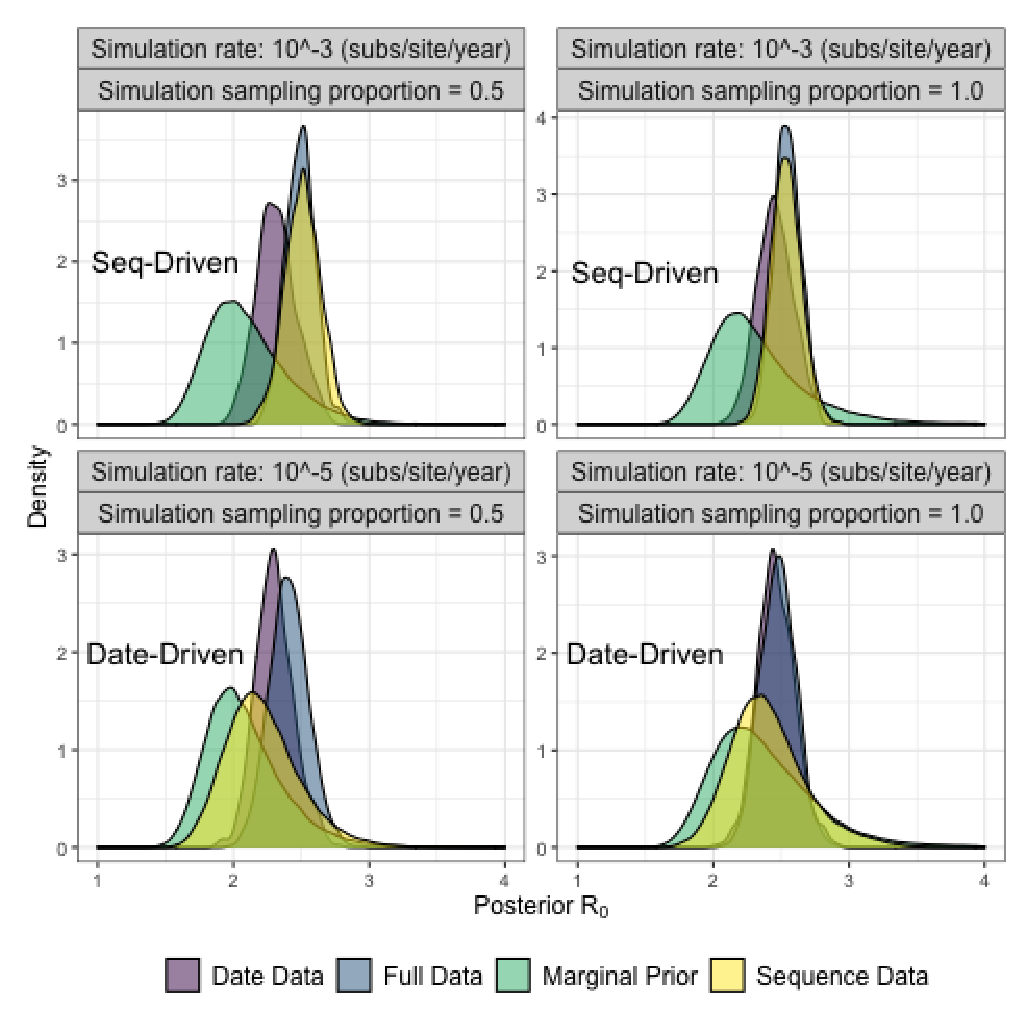
\includegraphics[width=1\linewidth]{../figures/postEg.eps}
\caption{\textcolor{blue}{Comparison of full data, date data, sequence data, and no data posterior $R_0$ for four of the 600 simulated datasets. \iffalse Tree 8 gives an example of when both date and sequence posteriors are similar while differing from the full data posterior. Here, $r_{SD}$ is higher, while $d_{SD}$ is lower such that classification using the Waserstein metric is both less meaningful and more likely to reflect noise due to MCMC sampling.\fi}}
\label{fig:posts}
\end{figure}
%---------------------------------------------------------------------------------------------------------
\subsection*{Reliability of Wasserstein Metric}

\textcolor{blue}{Section NEEDS: better clarification of subsampling validation and better description in general.}

Alignments were simulated under three sampling conditions ($p=0.05$, $p=0.5$, and $p=1$) to test robustness with respect to sampling proportion. We found that sampling proportion does not bias the distribution of the Wasserstein statistic between analyses (Fig \ref{fig:wData} D). This supports the assumption that comparing Wasserstein distance between analyses captures different signals concealed in date and sequence data. 

We also tested the accuracy of classification using the Wasserstein metric by subsampling and reclassifying each posterior $R_0$ distribution 100 times. Only 329 of resulting 40000 subsampled posteriors were misclassified  across 17 of the 400 datasets (\ref{fig:validateW}). Misclassififcation only occurred for datasets where $d_{SD}$ was below $10^{-1.47}$. Smaller $d_{SD}$ values indicate that the effect size of date and sequence data is similar and classification is not therefore not useful.

\begin{figure}[H]
\centering
\includegraphics[width=1\linewidth]{../figures/wassPanel.eps}
\caption{\textcolor{blue}{ \textbf{A}) Each point represents $(W_D, W_S)$ for one of the 600 simulated datasets with marginal histograms corresponding to the distribution of $W_D$ and $W_S$ respectively. \textbf{B}) The number of simulated datasets classified as Date of Seq Driven, stratified by evolutionary rate and sampling proportion. \textbf{C}) Points coloured by number of site patterns. Lower site patterns tends to co-occur with date-driven classification. \textbf{D}) Points coloured by date span with no clear patterns corresponding with classification as for site patterns. }}
\label{fig:wData}
\end{figure}

\subsection*{Observations about the effects of Sequence and Dates}
The distributions of $W_S$ is more diffuse than $W_D$, meaning the sequence data posterior tends to differ more from full data than date data (Fig \ref{fig:wData} A). This again aligns with previous results showing that date data drive inference under the birth-death.

Low sequence diversity, measured here in the number of site patterns, seems to preclude sequence data from driving inference (Fig \ref{fig:wData}B, Fig \ref{fig:patterns}). This matches the expectation that fewer site patterns results in less sequence information to inform the posterior. On the other hand, the date span  does not follow an equivalent trend with lower diversity coinciding with analyses being sequence driven. Here the relative date span is the time between the first and last sample, divided by the height of the outbreak tree and thus should be indicative of the information content of the dates. The distribution of relative date-span appears random across classifications, unlike the distribution of site patterns (Fig \ref{fig:wData}B, \ref{fig:patterns}).

%---------------------------------------------------------------------------------------------------------
\subsection*{Empirical Results}
We analysed data from two SARS-CoV-2 transmission clusters from 2020 in Australia to demonstrate that date-driven and sequence-driven analyses can arise in practice (table \ref{tab:tab2}). The first cluster is classified as sequence-driven, with $r_{SD} = 0.223$ indicating an appreciable difference between the sequence posterior and complete data. $d_{SD} = 0.078$ adds that date data also drives an effect of similar size, offering the interpretation that both date and sequence data are influential in this analysis. The second cluster is  classified as date-driven, but with $r_{SD} = 0.009$ and $d_{SD}=0.008$. The low $r_{SD}$ value indicates a near-negligible difference between date, sequence, and complete data posteriors. Since $r_{SD}$ is low, $d_{SD}$ is necessarily also low. Due to this, classification is effectively meaningless and it can be concluded that both date and sequence data drive a highly congruent signal. Moreover, $W_N$ for both analyses is more than double each of $W_S$ and $W_D$, which affirms that both sources of data contribute to the posterior deviating from the prior and are therefore informative with respect to the prior in both analyses.

\begin{table}[H]
\centering
\caption{Empirical data}
\begin{tabular}{lrr}
                    &   Cluster 1      &   Cluster 2     \\
\midrule
n                   &   112             &   188             \\
Classification      &   Seq-Driven       &   Date-Driven    \\
$r_{SD}$          &   0.223            &   0.009          \\
$d_{SD}$          &   0.078           &   0.008          \\
%Site-Patterns       &   -                &   -              \\
%Date-Patterns       &   -                &   -              \\
$W_{D}$             &   0.192            &   0.001          \\
$W_{S}$             &   0.114            &   0.009          \\
$W_{N}$             &   0.325            &   0.481          \\
\bottomrule 
\label{tab:tab2}
\end{tabular}
\end{table}
%---------------------------------------------------------------------------------------------------------
%---------------------------------------------------------------------------------------------------------
\section*{Discussion}
\textcolor{blue}{\subsection{Practical Implications}
    \begin{itemize}
        \item Need to curate date data as carefully as we do sequence data
        \item Points about clock and identifiability (chat with Seb)
        \item Usability of new methods and wasserstein to look at effects of data in future analyses. As we saw, the whole is not the sum of the parts, so best to look at the signal encoded in each
        \item Possibility of fixing the tree
        \item Maybe: Use for other parameters??
    \end{itemize}
    }
    
\textcolor{blue}{\subsection{Future Directions}
    \begin{itemize}
        \item Optimal Sampling: Need a way to judge what is optimal, assay the effects of sampling strategies
        \item Quality control new methods - e.g. cancer/ developmental phylodynamics where we have control over mutability and sampling time points
        \item Need some kind of statement about trends in sizes of phyloydnamics datasets, and non-linear increase with state space of inference
        \item Predictive way of classifiying information - clock is one way
    \end{itemize}
    }
The results of our simulation study add clarity to previous work showing that sampling times contribute substantially to phylodynamic inference under the birth death \citep{volz_sampling_2014, Featherstone2021Infectious}. We demonstrate that lower sequence diversity often precludes sequence data from a comparable effect. We also demonstrate that sequence data are not always secondary in influence and can drive inference of $R_{0}$ in some instances, affirming the sensitivity of the birth-death to the signal encoded in sequence data. The tendency for date data to drive inference more than sequence data may be explained by the reduction in uncertainty that each data source offers. Dates impose a hard bound on topology by restricting tree space to a subset of topologies that agree with the chronology of sampling times. Conversely, sequence data inform topology through phylogenetic likelihood, but do not definitively constrain tree space in the same way as date data.

Our method offers novel insight for phylodynamics practitioners because the contribution of sequence data relative to sampling dates is often questioned in birth death analyses of densely sequenced outbreaks. It offers a reproducible approach to answering this question so the influence of genomic data can be commented on. For example, this is useful in a public health reporting context so phylodynamics experts can comment on the drivers inference as new data emerge. As such it offers a tool to initiate research into optimal sampling design for phylodynamic analysis. Any resulting theory can only be speculative at best, given the unpredictable nature of evolution, however this is an important consideration for the future as the scale of pathogen genome sequencing increases.

%This main limitation of our method is that it requires phylodnamic analysis to generate results, rather than taking sampling times and sequence as sole inputs. However, given the complex expression for phylodynamic likelihood under the birth death, it is unlikely that such a predictive method is analytically achievable, and is certainly beyond the scope of this study.
%---------------------------------------------------------------------------------------------------------
%---------------------------------------------------------------------------------------------------------
\subsection*{Data Archival}
All scripts used to simulate and analyse data are available at \url{https://github.com/LeoFeatherstone/phyloDataSignal.git}. The Feast package, containing our date estimator, is available at \url{https://github.com/tgvaughan/feast.git}.
%---------------------------------------------------------------------------------------------------------
%---------------------------------------------------------------------------------------------------------
\section*{Methods}
\subsection*{Simulation Study}
We simulated 100 outbreaks of 500 cases under a birth death process using the \url{Tree-Sim} R package \citep{TreeSim}. The birth rate was set to $2.5$, death rate $1$, corresponding to $R_{0} = 2.5$. \textcolor{blue}{Sampling probability was set to $p=1$, resulting in trees with 500 tips.} We then extended this to a set of 300 outbreaks by sampling again with probability $p=0.05$ and $p = 0.5$, resulting in trees of 25 and 50 tips. We used a consistent seed such that each outbreak with $p=0.05$ or $p=0.5$ corresponds to a subsample of another with $p=1$, allowing us to asses the effect of sampling proportion on inferring $W_{\bullet}$. For each outbreak, we used Seq-Gen to sequence alignments of length 20000, which is roughly average for RNA viruses \citep{sanjuan2010viral,rambaut_seq-gen_1997}. We set an Jukes-Cantor model with evolutionary rate set to either $10^{-3}$ or $10^-{5}$ subs/site/time using Seq-Gen \cite{rambaut_seq-gen_1997}.  Our choice of evolutionary rates allows us to compare the effects higher and lower sequence information with the former corresponding to about 20 substitutions per infection, and 0.2 for the latter. 
The above resulted in 600 alignments to test in the four treatments described above. We analysed each under a birth-death model using BEAST v2.6 \citet{bouckaert_beast_2019} with a $\textrm{Uniform}[0,5]$ prior for $R_0$ and all other parameters set to the true value for simplicity and to disentangle any impacts of parameter nonidentifiability \citep{louca2021fundamental}.

\subsection*{Empirical Data}
We analysed two similar SARS-CoV-2 datasets taken from \citet{lane2021genomics}. They consisted of 112 and 188 samples respectively. \textcolor{blue}{These clusters were chosen out of the 595 identified by \citet{lane2021genomics} because they possessed the most complete sampling-time data to compare with sequence data. They are also ideal examples of the size and type of genome dataset that public health practitioners may seek phylodynamic insight from as the sample most likely reflects transmission stemming from a single, unknown source.} 

We analysed  each dataset under the four conditions above. In each, we placed a $\textrm{Lognormal}(\textrm{mean}=1, \textrm{sd}=1.25)$ prior on $R_0$ and an $\textrm{Inv-Gamma}(\alpha=5.807, \beta=346.020)$ prior on the becoming-uninfectious rate ($\delta$) following estimates of the duration of infection ($=\frac{1}{\delta}$) in \cite{Lauer2020The}. \textcolor{blue}{We also fixed the sampling proportion to $p=0.8$ since every known Victorian SARS-CoV-2 case was sequenced at this stage of the pandemic, with a roughly 20\% sequencing failure rate.} We also placed an $\textrm{Exp}(\textrm{mean}=0.019)$ prior on the origin, corresponding to a lag of up to one week  between the index case and the first putative transmission event.

\subsection*{Calculating and Validating the Wasserstein Metric}
We used the \href{https://www.rdocumentation.org/packages/transport/versions/0.12-2/topics/wasserstein1d}{\textcolor{blue}{transport}} R package to calculate the Wasserstein metric. 

\textcolor{blue}{We conducted a subsampling analysis to ensure that Wasserstein metric values reflected differences between date and sequence data, rather than noise alone. For each of the 600 simulated datasets, we subsampled posterior $R_{0}$ distributions corresponding to each data treatment 100 times, taking a number of samples equal to half the length of the post-burnin posterior. This resulted in a dataset of 60,000 subsampled posteriors for which we re-calcualted Wasserstein values and reclassified each as in the original simulation study. Of the 60,000, subsampled posteriors, only 99 were misclassified across 99 of the 600 original datasets. In other words, misclassification occurred only once for 99 of the 600 simulated datasets.}

\textcolor{blue}{Of the 600 simulated datasets, those where misclassification occurred had substantially smaller differences between Wasserstein distance to the date-only and sequence-only posteriors ($d_{SD}$) (Figure \ref{fig:validateW}). Misclassification occurred where $d_{SD} \le 8.27\times10^{-2}$ in the complete $R_0$ posteriors, with no error above this level. Differences below $8.27\times10^{-2}$ correspond to a level of difference between data and sequence only posteriors where classification is of little significance (i.e. $R_0 \pm 0.08$ assuming both posteriors have similar uncertainty). Classification is wholly reliable above this threshold, validating the trends observed in the simulation study.}

\renewcommand{\thefigure}{S\arabic{figure}}
\setcounter{figure}{0}

\begin{figure}[H]
\centering
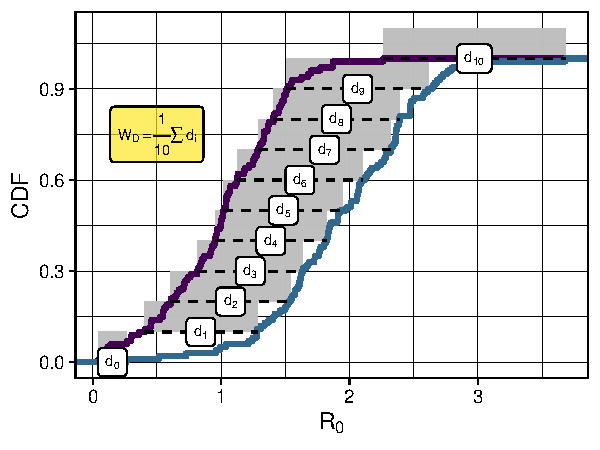
\includegraphics[width=0.5\linewidth]{../figures/wassersteinIntuition.eps}
\caption{\textcolor{blue}{ MAYBE CITE CS-PAPER. Visual intuition for calculation of the wasserstein metric. It can be thought of as integration over the horizontal distance between points of the cumulative distribution function. For two sets of posterior samples from an MCMC, the 10 horizontal distances would be replaced by the the size of the greatest set of samples.}}
\label{fig:wassIntuition}
\end{figure}

\begin{figure}[H]
\centering
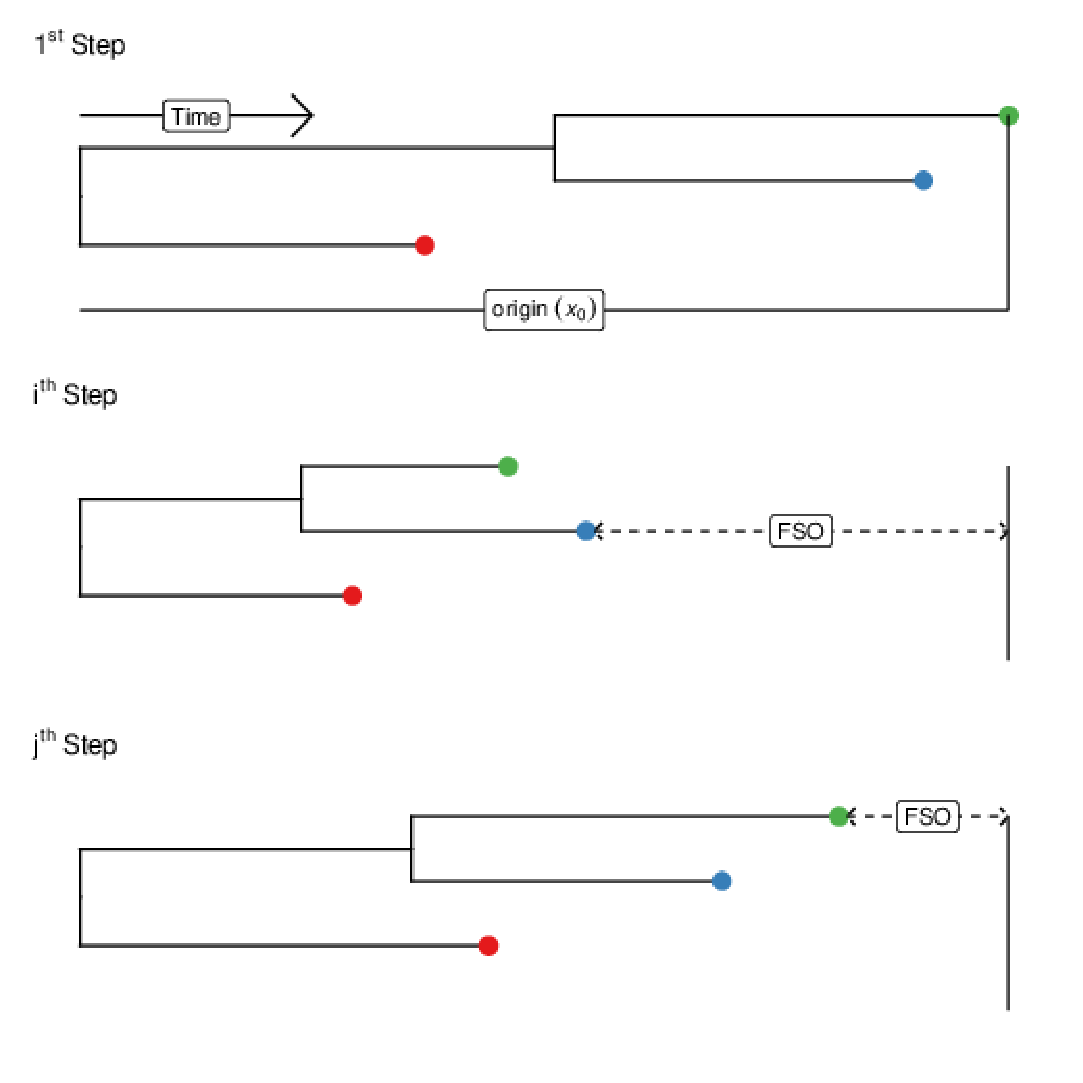
\includegraphics[width=1\linewidth]{../figures/tipDateOp.eps}
\caption{\textcolor{blue}{Visual intuition for the novel tip-date operator that allows for inference from sequence only datasets. Each row represents a state in an hypothetical MCMC chain. The Final Sample Offset (FSO) is the time between the final sample and the theoretical end of the proposed birth-death process. It is normally held constant in inference. The tip date operator allows for new proposals of the FSO which allows tip dates to rescale relative one each other and in absolute time. The origin time does not contain the FSO.}}
\label{fig:tipOp}
\end{figure}

\begin{figure}[H]
\centering
\includegraphics[width=1\linewidth]{../figures/postMCITreeDist.eps}
\caption{\textcolor{blue}{Violin plots of pairwise mutual clustering information tree difference for 100 trees sampled posterior tree distributions for each simulated dataset. 100 trees were samples from each of the 600 posterior tree distributions a total of 100 times, resulting in 60,000 datapoints here, separated by the sampling proportion and evolutionary rate used in each simulation. Uniformly, Full data has the least tree-distance between posterior trees followed by the sequence-only, dates-only, and no-data treatments.}}
\label{fig:ptreeDist}
\end{figure}

\begin{figure}[H]
\centering
\includegraphics[width=0.75\linewidth]{../figures/egTreeSpace.eps}
\caption{\textcolor{teal}{Note, I was really wrong in my earlier thinking about there being a different numbr of of topologies for each data source. I will need to revisit this when writing the paper. }\textcolor{blue}{Tree space for a tree with 3 taxa. There are a total of 18 possible ranked topologies, which would be the size of tree space for an analyses of a sequence-only dataset with tree samples. Trees in blue are those with the sampling chronology A, B, and then C. These represent the tree space for a hypothetical data-only dataset with three sampling times. Moreover, the disparity between the sequence-only tree space and date-only space grows with sample size, such that the state-space for sequence-only data is orders of magnitude larger than that for dates-only}}
\label{fig:treeSpace}
\end{figure}


\begin{figure}[H]
\centering
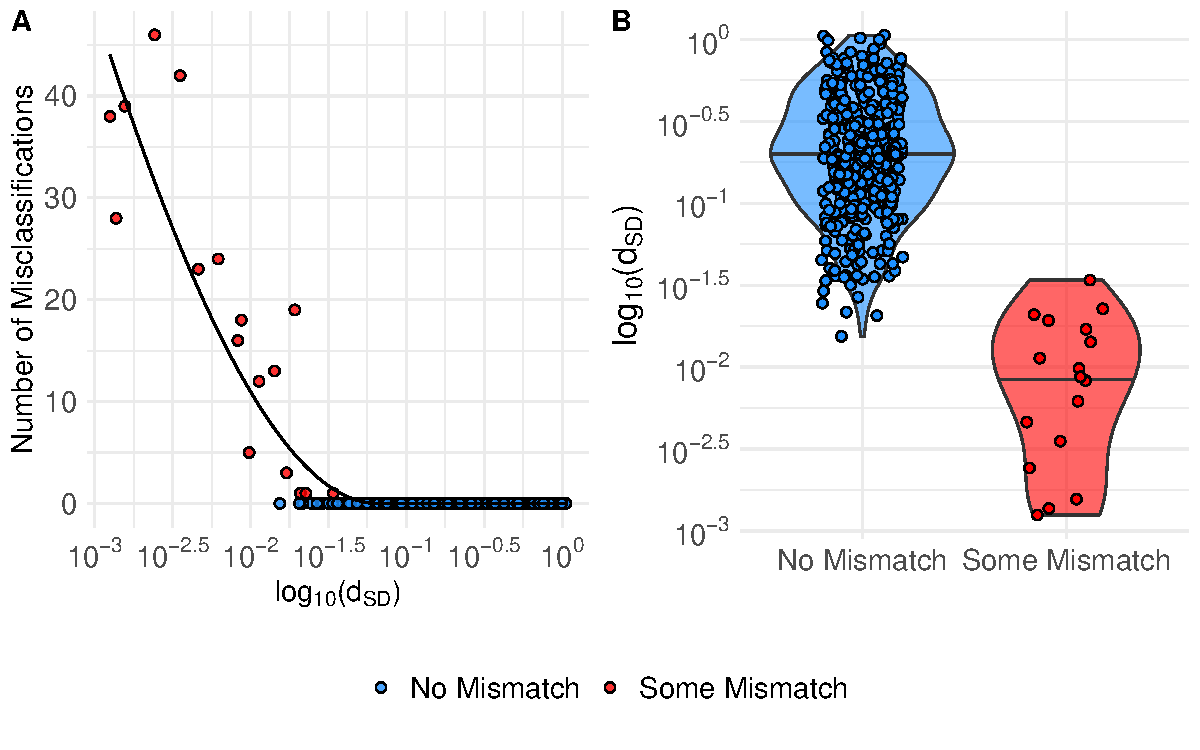
\includegraphics[width=1\linewidth]{../figures/errorWasserstein.eps}
\caption{ \textbf{A}) Each point presents the number of misclassification in subsampling posterior $R_0$ for each of the 600 simulated datasets. X-axis is the log transformed difference between $W_S$ and $W_D$. \textbf{B}) Violin plots with jittered points of the difference between $W_S$ and $W_D$ for simulated alignments where there was wither some one no misclassification. Both \textbf{A} and \textbf{B} support that misclassication only occurs where the difference between $W_S$ and $W_D$ is negligible, and classification is not meaningful in the first instance.}
\label{fig:validateW}
\end{figure}

\begin{figure}[H]
\centering
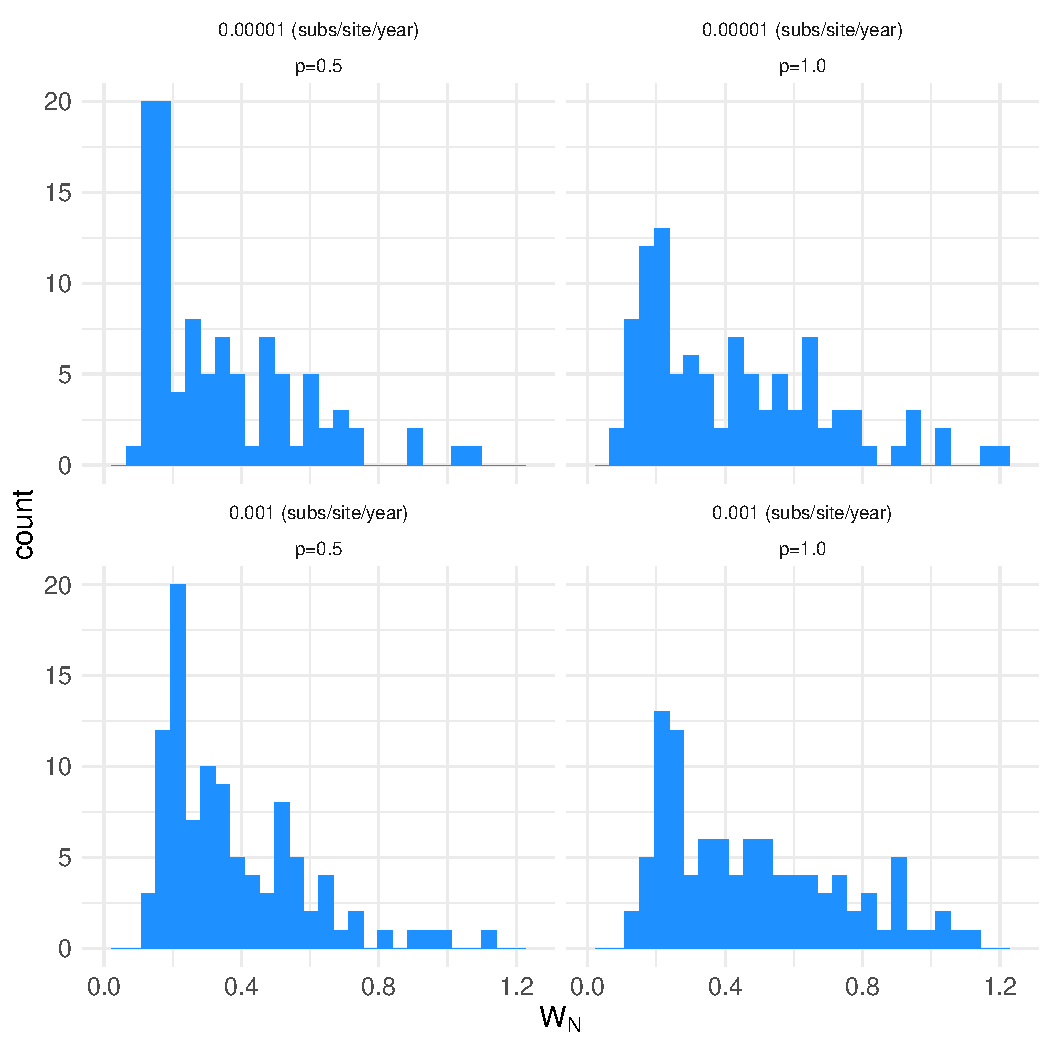
\includegraphics[width=1\linewidth]{../figures/wnHist.eps}
\caption{Histogram of $W_N$ for each simulated dataset, separated by evolutionary rate and sampling proportion. $W_N$ ranges from 0.06 to 1.02, such that simulated data provide additional information beyond that of the prior in each analysis.}
\label{fig:wnHist}
\end{figure}

\begin{figure}[H]
\centering
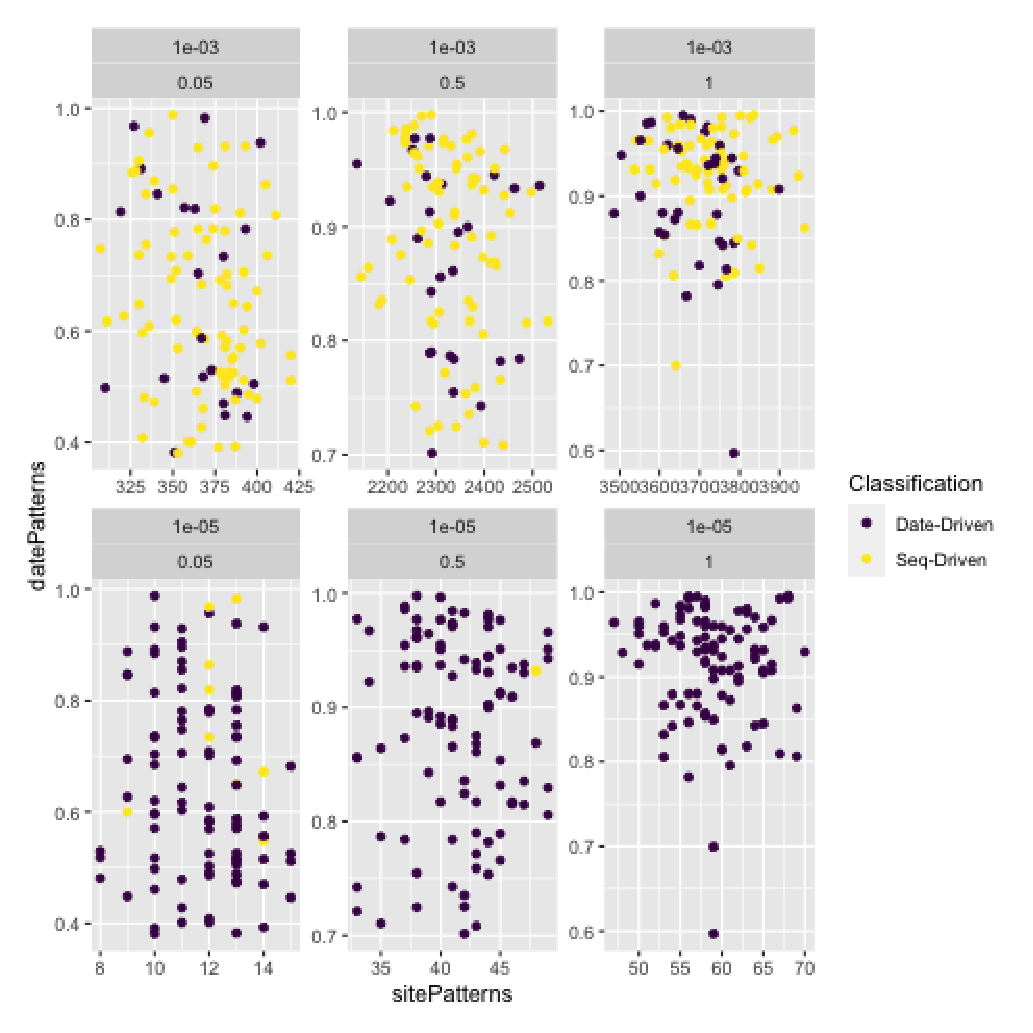
\includegraphics[width=1\linewidth]{../figures/patternsClass.eps}
\caption{Date patterns ($=\frac{\text{Sampling Span}}{\text{Height}}$) against site patterns for each simulated dataset. Plots are separated by evolutionary rate and sampling proportion such that there are 600 points coloured by Wasserstein Classification across the entire figure. Higher evolutionary rates increase the proportion of Sequence driven datasets, but within each rate there is no clear pattern in date patterns, site patterns, or sampling rate driving classification.}
\label{fig:patterns}
\end{figure}

%---------------------------------------------------------------------------------------------------------
%---------------------------------------------------------------------------------------------------------
\section*{Acknowledgements}
LAF is grateful to Swissnex for awarding a Student Research Scholarship to foster this research. SD and LAF were received funding from the Australian Research Council (DE190100805), the Australian Medical Research Futures Fund (MRF9200006), and the National Health and Medical Research Council (APP1157586)
%---------------------------------------------------------------------------------------------------------
%---------------------------------------------------------------------------------------------------------
%\bibliographystyle{natbib}
\bibliography{refs}%%%bibliography file(.bib)
%---------------------------------------------------------------------------------------------------------
%---------------------------------------------------------------------------------------------------------
\end{document}
